
%{{第二十三回}}{第二十三回}}

\chapter{西厢记妙词通戏语\hspace{.5em}牡丹亭艳曲警芳心}
{  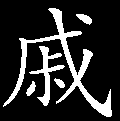
\includegraphics[width=3mm]{../Images/00005}群艳大观中,柳弱系轻风。惜花与度曲,笑看利名空。}

话说贾元春自那日幸大观园回宫去后,便命将那日所有的题咏,命探春依次抄录妥协,自己编次,叙其优劣,又命在大观园勒石,为千古风流雅事。因此,贾政命人各处选拔精工名匠,在大观园磨石镌字,贾珍率领蓉、萍等监工。因贾蔷又管理着文官等十二个女戏并行头等事,不大得便,因此贾珍又将贾菖、贾菱唤来监工。一日,烫蜡钉朱,动起手来。这也不在话下。

且说那个玉皇庙并达摩庵两处,一班的十二个小沙弥并十二个小道士,如今挪出大观园来,贾政正想发到各庙去分住。不想后街上住的贾芹之母周氏,正盘算着也要到贾政这边谋一个大小事务与儿子管管,也好弄些银钱使用,可巧听见这件事出来,便坐轿子来求凤姐。凤姐因见他素日不大拿班作势的,便依允了,想了几句话{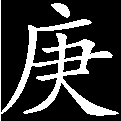
\includegraphics[width=3mm]{../Images/00004}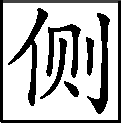
\includegraphics[width=3mm]{../Images/00011}\footnotesize \kaishu 一派心机。}便回王夫人说:``这些小和尚道士万不可打发到别处去,一时娘娘出来就要承应。倘或散了,若再用时,可是又费事。依我的主意,不如将他们竟送到咱们家庙里铁槛寺去,月间不过派一个人拿几两银子去买柴米就完了。说声用,走去叫来,一点儿不费事呢。''王夫人听了,便商之于贾政。贾政听了笑道:``倒是提醒了我,就是这样。''即时唤贾琏来。

当下贾琏正同凤姐吃饭,一闻呼唤,不知何事,放下饭便走。凤姐一把拉住,笑道:``你且站住,听我说话。若是别的事我不管,若是为小和尚们的事,好歹依我这么着。''如此这般教了一套话。贾琏笑道:``我不知道,你有本事你说去。''凤姐听了,把头一梗,把筷子一放,{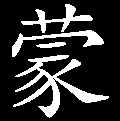
\includegraphics[width=3mm]{../Images/00006}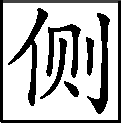
\includegraphics[width=3mm]{../Images/00011}\footnotesize \kaishu 活跳。}腮上似笑不笑的瞅着贾琏道:``你当真的,是玩话?''贾琏笑道:``西廊下五嫂子的儿子芸儿来求了我两三遭,{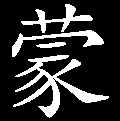
\includegraphics[width=3mm]{../Images/00006}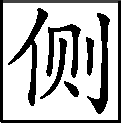
\includegraphics[width=3mm]{../Images/00011}\footnotesize \kaishu 可发一笑。}要个事情管管。我依了,叫他等着。好容易出来这件事,你又夺了去。''凤姐儿笑道:``你放心。园子东北角子上,娘娘说了,还叫多多的种松柏树,楼底下还叫种些花草。等这件事出来,我管保叫芸儿管这件工程。''贾琏道:``果然这样也罢了。只是昨儿晚上,我不过是要改个样儿,你就扭手扭脚的。''{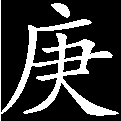
\includegraphics[width=3mm]{../Images/00004}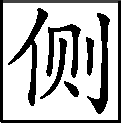
\includegraphics[width=3mm]{../Images/00011}\footnotesize \kaishu 写凤姐风月之文如此,总不脱漏。}凤姐儿听了,``嗤''的一声笑了,{{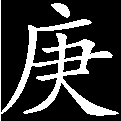
\includegraphics[width=3mm]{../Images/00004}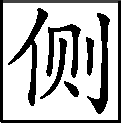
\includegraphics[width=3mm]{../Images/00011}\footnotesize \kaishu 好章法! }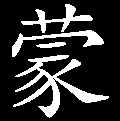
\includegraphics[width=3mm]{../Images/00006}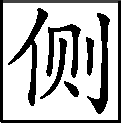
\includegraphics[width=3mm]{../Images/00011}\footnotesize \kaishu 粗蠢,情景可笑。后将有大观园中一段奇情韵{[}事{]},不得不先为此等丑语一跌,以作未火先烟之象。}向贾琏啐了一口,低下头便吃饭。贾琏已经笑着去了。

到了前面,见了贾政,果然是小和尚一事。贾琏便依了凤姐主意,说道:``如今看来,芹儿倒大大的出息了,这件事竟交予他去管办。横竖照在里头的规例,每月叫芹儿支领就是了。''贾政原不大理论这些事,听贾琏如此说,便如此依了。贾琏回到房中告诉凤姐儿,凤姐即命人去告诉了周氏。贾芹便来见贾琏夫妻两个,感谢不尽。凤姐又作情央贾琏先支三个月的,叫他写了领字,贾琏批票画了押,登时发了对牌出去。银库上按数发出三个月的供给来,白花花二三百两。贾芹随手拈一块,撂与掌平的人,叫他们吃了茶罢。于是命小厮拿回家,与母亲商议。登时雇了大叫驴,自己骑上,又雇了几辆车,至荣国府角门,唤出二十四个人来,坐上车,一径往城外铁槛寺去了。当下无话。

如今且说贾元春,因在宫中自编大观园题咏之后,忽想起那大观园中景致,自己幸过之后,贾政必定敬谨封锁,不敢使人进去骚扰,岂不寥落。况家中现有几个能诗会赋的姊妹,何不命他们进去居住,也不使佳人落魄,花柳无颜。{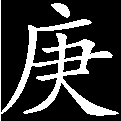
\includegraphics[width=3mm]{../Images/00004}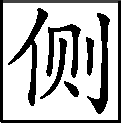
\includegraphics[width=3mm]{../Images/00011}\footnotesize \kaishu 韵人行韵事。}却又想到宝玉自幼在姊妹丛中长大,{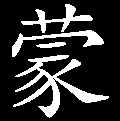
\includegraphics[width=3mm]{../Images/00006}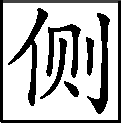
\includegraphics[width=3mm]{../Images/00011}\footnotesize \kaishu 何等精细!}不比别的兄弟,若不命他进去,只怕他冷清了,一时不大畅快,未免贾母、王夫人愁虑,须得也命他进园居住方妙。{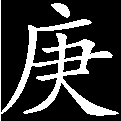
\includegraphics[width=3mm]{../Images/00004}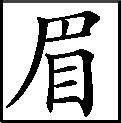
\includegraphics[width=3mm]{../Images/00010}\footnotesize \kaishu 大观园原系十二钗栖止之所,然工程浩大,故借元春之名而起,再用元春之命以安诸艳,不见一丝扭捻。己卯冬夜。}想毕,遂命太监夏守忠到荣国府来下一道谕,命宝钗等只管在园中居住,不可禁约封锢,命宝玉仍随进去读书。

贾政、王夫人接了这谕,待夏守忠去后,便来回明贾母,遣人进去各处收拾打扫,安设帘幔床帐。别人听了还自犹可,惟宝玉听了这谕,喜的无可不可。正和贾母盘算,要这个,弄那个,忽见丫鬟来说:``老爷叫宝玉。''{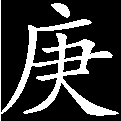
\includegraphics[width=3mm]{../Images/00004}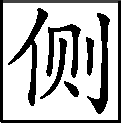
\includegraphics[width=3mm]{../Images/00011}\footnotesize \kaishu 多大力量写此句。余亦惊骇,况宝玉乎!回思十二三时,亦曾有是病来。想时不再至,不禁泪下。}宝玉听了,{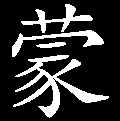
\includegraphics[width=3mm]{../Images/00006}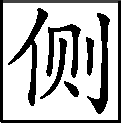
\includegraphics[width=3mm]{../Images/00011}\footnotesize \kaishu 大家风范!}好似打了个焦雷,登时扫去兴头,脸上转了颜色,便拉着贾母扭的好似扭股儿糖,杀死不敢去。贾母只得安慰他道:``好宝贝,你只管去,有我呢,他不敢委屈了你。{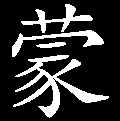
\includegraphics[width=3mm]{../Images/00006}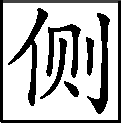
\includegraphics[width=3mm]{../Images/00011}\footnotesize \kaishu 写尽祖母溺爱,作后文之本!}况且你又作了那篇好文章。想是娘娘叫你进去住,他吩咐你几句,不过不教你在里头淘气。他说什么,你只好生答应着就是了。''一面安慰,一面唤了两个老嬷嬷来,吩咐:``好生带了宝玉去,别叫他老子唬着他。''老嬷嬷答应了。

宝玉只得前去,一步挪不了三寸,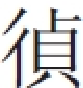
\includegraphics[width=4mm]{../images/00015}{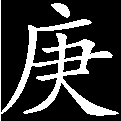
\includegraphics[width=3mm]{../Images/00004}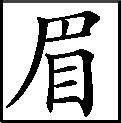
\includegraphics[width=3mm]{../Images/00010}\footnotesize \kaishu 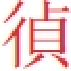
\includegraphics[width=3mm]{../images/00016},撑去声。}到这边来。可巧贾政在王夫人房中商议事情,金钏儿、彩云、彩霞、绣鸾、绣凤等众丫鬟都在廊檐底下站着呢,一见宝玉来,都抿着嘴笑。金钏一把拉住宝玉,{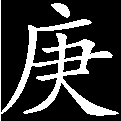
\includegraphics[width=3mm]{../Images/00004}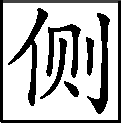
\includegraphics[width=3mm]{../Images/00011}\footnotesize \kaishu 有是事,有是人。}悄悄的笑道:``我这嘴上是才擦的香浸胭脂,{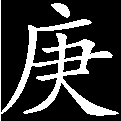
\includegraphics[width=3mm]{../Images/00004}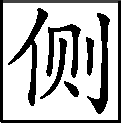
\includegraphics[width=3mm]{../Images/00011}\footnotesize \kaishu 活像活现。}你这会子可吃不吃了?''彩云一把推开金钏,笑道:``人家正心里不自在,你还奚落他。趁这会子喜欢,快进去罢。''宝玉只得挨进门去。原来贾政和王夫人都在里间呢。赵姨娘打起帘子,宝玉躬身进去。只见贾政和王夫人对面坐在炕上说话,地下一溜椅子,迎春、探春、惜春、贾环四个人都坐在那里。一见他进来,惟有探春和惜春、贾环站了起来。

贾政一举目,见宝玉站在跟前,神彩飘逸,秀色夺人,{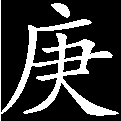
\includegraphics[width=3mm]{../Images/00004}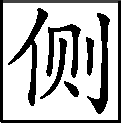
\includegraphics[width=3mm]{../Images/00011}\footnotesize \kaishu ``消气散''用的好。}看看贾环,人物委琐,举止荒疏,忽又想起贾珠来,{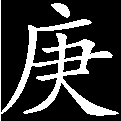
\includegraphics[width=3mm]{../Images/00004}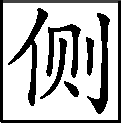
\includegraphics[width=3mm]{../Images/00011}\footnotesize \kaishu 批至此,几乎失声哭出。}再看看王夫人只有这一个亲生的儿子,素爱如珍,自己的胡须将已苍白:因这几件上,把素日嫌恶处分宝玉之心不觉减了八九。{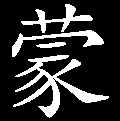
\includegraphics[width=3mm]{../Images/00006}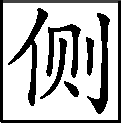
\includegraphics[width=3mm]{../Images/00011}\footnotesize \kaishu 为天下年老者父母一哭!}半晌说道:``娘娘吩咐说,你日日外头嬉游,渐次疏懒,如今叫禁管,{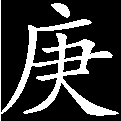
\includegraphics[width=3mm]{../Images/00004}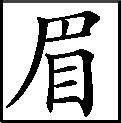
\includegraphics[width=3mm]{../Images/00010}\footnotesize \kaishu 写宝玉可入园,用``禁管''二字,得体,理之至。壬午九月。}同你姊妹在园里读书写字。你可好生用心习学,再如不守分安常,你可仔细!''宝玉连连的答应了几个``是''。王夫人便拉他在身旁坐下。{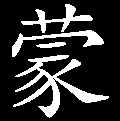
\includegraphics[width=3mm]{../Images/00006}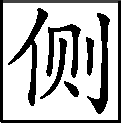
\includegraphics[width=3mm]{../Images/00011}\footnotesize \kaishu 活现!}他姊弟三人依旧坐下。

王夫人摸挲着宝玉的脖项说道:``前儿的丸药都吃完了?''宝玉答道:``还有一丸。''王夫人道:``明儿再取十丸来,天天临睡的时候,叫袭人伏侍你吃了再睡。''宝玉道:``只从太太吩咐了,袭人天天晚上想着,打发我吃。''{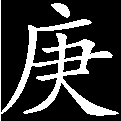
\includegraphics[width=3mm]{../Images/00004}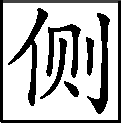
\includegraphics[width=3mm]{../Images/00011}\footnotesize \kaishu 大家细细听去,活似小儿口气。}贾政问道:``袭人是何人?''王夫人道:``是个丫头。''贾政道:``丫头不管叫个什么罢了,是谁这样刁钻,起这样的名字?''王夫人见贾政不自在了,便替宝玉掩饰道:``是老太太起的。''贾政道:``老太太如何知道这话,一定是宝玉。''宝玉见瞒不过,只得起身回道:``因素日读诗,曾记古人有一句诗云:`花气袭人知昼暖'\href{../Text/part0027_split_000.html\#lnkback_1_a}{\textsuperscript{①}}。因这个丫头姓花,便随口起了这个名字。''王夫人忙又道:``宝玉,你回去改了罢。老爷也不用为这小事动气。''贾政道:``究竟也无碍,又何用改。{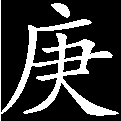
\includegraphics[width=3mm]{../Images/00004}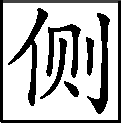
\includegraphics[width=3mm]{../Images/00011}\footnotesize \kaishu 几乎改去好名。}只是可见宝玉不务正,专在这些浓词艳赋上作工夫。''说毕,断喝一声:{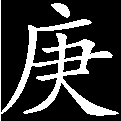
\includegraphics[width=3mm]{../Images/00004}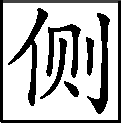
\includegraphics[width=3mm]{../Images/00011}\footnotesize \kaishu 好收拾。}``作业的畜生,还不出去!''王夫人也忙道:``去罢,只怕老太太等你吃饭呢。''{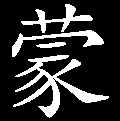
\includegraphics[width=3mm]{../Images/00006}\includegraphics[width=3mm]{../Images/00011}\footnotesize \kaishu 严父慈母,其事虽异,其行则一。}宝玉答应了,慢慢的退出去,向金钏儿笑着伸伸舌头,带着两个嬷嬷一溜烟去了。

刚至穿堂门前,{\includegraphics[width=3mm]{../Images/00004}\includegraphics[width=3mm]{../Images/00012}\footnotesize \kaishu 妙!这便是凤姐扫雪拾玉之处,一丝不乱。}只见袭人倚门立在那里,{\includegraphics[width=3mm]{../Images/00006}\includegraphics[width=3mm]{../Images/00011}\footnotesize \kaishu 何等牵连!}一见宝玉平安回来,堆下笑来问{\includegraphics[width=3mm]{../Images/00004}\includegraphics[width=3mm]{../Images/00011}\footnotesize \kaishu 等坏了,愁坏了。所以有``堆下笑来问''之话。}道:``叫你作什么?''宝玉告诉他:``没有什么,不过怕我进园去淘气,吩咐吩咐。''{\includegraphics[width=3mm]{../Images/00004}\includegraphics[width=3mm]{../Images/00011}\footnotesize \kaishu 就说大话,毕肖之至!}一面说,一面回至贾母跟前,回明原委。只见林黛玉正在那里,宝玉便问他:``你住那一处好?''林黛玉正心里盘算这事,{\includegraphics[width=3mm]{../Images/00004}\includegraphics[width=3mm]{../Images/00011}\footnotesize \kaishu 颦儿亦有盘算事,拣择清幽处耳,未知择邻否?一笑。}忽见宝玉问他,便笑道:``我心里想着潇湘馆好,爱那几竿竹子隐着一道曲栏,比别处更觉幽静。''宝玉听了拍手笑道:``正和我的主意一样,我也要叫你住这里呢。我就住怡红院,咱们两个又近,又都清幽。''{{\includegraphics[width=3mm]{../Images/00004}\includegraphics[width=3mm]{../Images/00011}\footnotesize \kaishu 择邻出于玉兄,所谓真知己。 }\includegraphics[width=3mm]{../Images/00006}\includegraphics[width=3mm]{../Images/00011}\footnotesize \kaishu 作后文无限张本。}

二人正计较,就有贾政遣人来回贾母说:``二月二十二,日子好,哥儿姐儿们好搬进去的。这几日内遣人进去分派收拾。''薛宝钗住了蘅芜苑,林黛玉住了潇湘馆,贾迎春住了缀锦楼,探春住了秋爽斋,\href{../Text/part0027_split_000.html\#lnkback_2_a}{\textsuperscript{②}}惜春住了蓼风轩,李氏住了稻香村,宝玉住了怡红院。每一处添两个老嬷嬷,四个丫头,除各人奶娘亲随丫鬟不算外,另有专管收拾打扫的。至二十二日,一齐进去,登时园内花招绣带,柳拂香风,{\includegraphics[width=3mm]{../Images/00004}\includegraphics[width=3mm]{../Images/00012}\footnotesize \kaishu 八字写得满园之内处处有人,无一处不到。}不似前番那等寂寞了。

闲言少叙。且说宝玉自进花园以来,心满意足,再无别项可生贪求之心。每日只和姊妹、丫头们一处,或读书,{\includegraphics[width=3mm]{../Images/00004}\includegraphics[width=3mm]{../Images/00011}\footnotesize \kaishu 未必。}或写字,或弹琴下棋,作画吟诗,以至描鸾刺凤,{\includegraphics[width=3mm]{../Images/00004}\includegraphics[width=3mm]{../Images/00011}\footnotesize \kaishu 有之。}斗草簪花,低吟悄唱,拆字猜枚,无所不至,倒也十分快乐。他曾有几首即事诗,虽不算好,却倒是真情真景,略记几首云:

春夜即事

霞绡云幄任铺陈,隔巷蟆更听未真。

枕上轻寒窗外雨,眼前春色梦中人。

盈盈烛泪因谁泣,默默花愁为我嗔。

自是小鬟娇懒惯,拥衾不耐笑言频。

夏夜即事

倦绣佳人幽梦长,金笼鹦鹉唤茶汤。

窗明麝月开宫镜,室霭檀云品御香。

琥珀杯倾荷露滑,玻璃槛纳柳风凉。

水亭处处齐纨动,帘卷朱楼罢晚妆。

秋夜即事

绛芸轩里绝喧哗,桂魄流光浸茜纱。

苔锁石纹容睡鹤,井飘桐露湿栖鸦。

抱衾婢至舒金凤,倚槛人归落翠花。

静夜不眠因酒渴,沉烟重拨索烹茶。

冬夜即事

梅魂竹梦已三更,锦罽鹴衾睡未成。

松影一庭惟见鹤,梨花满地不闻莺。

女儿翠袖诗怀冷,公子金貂酒力轻。

却喜侍儿知试茗,扫将新雪及时烹。

{\includegraphics[width=3mm]{../Images/00004}\includegraphics[width=3mm]{../Images/00010}\footnotesize \kaishu 四诗作尽安福尊荣之贵介公子也。壬午孟夏。}

因这几首诗,当时有一等势利人,见是荣国府十二三岁的公子作的,抄录出来各处称颂,再有一等轻浮子弟,爱上那风骚妖艳之句,也写在扇头壁上,不时吟哦赏赞。因此竟有人来寻诗觅字,倩画求题的。宝玉亦发得了意,镇日家作这些外务。

谁想静中生烦恼,忽一日不自在起来,这也不好,那也不好,出来进去只是闷闷的。园中那些人多半是女孩儿,正在混沌世界,天真烂漫之时,坐卧不避,嬉笑无心,那里知宝玉此时的心事。那宝玉心内不自在,便懒在园内,只在外头鬼混,却又痴痴的。{\includegraphics[width=3mm]{../Images/00004}\includegraphics[width=3mm]{../Images/00012}\footnotesize \kaishu 不进园去,真不知何心事。}茗烟见他这样,因想与他开心,左思右想,皆是宝玉顽奈烦了的,不能开心,惟有这件,宝玉不曾看见过。{\includegraphics[width=3mm]{../Images/00004}\includegraphics[width=3mm]{../Images/00011}\footnotesize \kaishu 书房伴读累累如是,余至今痛恨。}想毕,便走去到书坊内,把那古今小说并那飞燕、合德、武则天、杨贵妃的外传与那传奇角本买了许多来,引宝玉看。宝玉何曾见过这些书,一看见了便如得了珍宝。茗烟嘱咐他不可拿进园去,{\includegraphics[width=3mm]{../Images/00006}\includegraphics[width=3mm]{../Images/00011}\footnotesize \kaishu 自古恶奴坏事。}``若叫人知道了,我就吃不了兜着走呢。''宝玉那里舍的不拿进去,踟蹰再三,单把那文理细密的拣了几套进去,放在床顶上,无人时自己密看。那粗俗过露的,都藏在外面书房里。

那一日,正当三月中浣,早饭后,宝玉携了一套《会真记》,走到沁芳闸桥边桃花底下一块石上坐着,展开《会真记》,从头细玩。正看到``落红成阵'',只见一阵风过,把树头上桃花吹下一大半来,{\includegraphics[width=3mm]{../Images/00004}\includegraphics[width=3mm]{../Images/00011}\footnotesize \kaishu 好一阵凑趣风。}落的满身满书满地皆是。宝玉要抖将下来,恐怕脚步践踏了,{\includegraphics[width=3mm]{../Images/00004}\includegraphics[width=3mm]{../Images/00012}\footnotesize \kaishu 情不情。}只得兜了那花瓣,来至池边,抖在池内。那花瓣浮在水面,飘飘荡荡,竟流出沁芳闸去了。

回来只见地下还有许多,宝玉正踟蹰间,只听背后有人说道:``你在这里作什么?''宝玉一回头,却是林黛玉来了,肩上担着花锄,锄上挂着花囊,手内拿着花帚。{{\includegraphics[width=3mm]{../Images/00004}\includegraphics[width=3mm]{../Images/00011}\footnotesize \kaishu 一幅采芝图,非葬花图也。 \includegraphics[width=3mm]{../Images/00004}\includegraphics[width=3mm]{../Images/00010}\footnotesize \kaishu 此图欲画之心久矣,誓不遇仙笔不写,恐亵我颦卿故也。己卯冬。 \includegraphics[width=3mm]{../Images/00004}\includegraphics[width=3mm]{../Images/00010}\footnotesize \kaishu 丁亥春间,偶识一浙省{[}新{]}发,其白描美人,真神品物,甚合余意。奈彼因宦缘所缠无暇,且不能久留都下,未几南行矣。余至今耿耿,怅然之至。恨与阿颦结一笔墨缘之难若此!叹叹!丁亥夏。畸笏叟。 }\includegraphics[width=3mm]{../Images/00006}\includegraphics[width=3mm]{../Images/00011}\footnotesize \kaishu 真是韵人韵事! \includegraphics[width=3mm]{../Images/00009}\includegraphics[width=3mm]{../Images/00012}\footnotesize \kaishu 写出扫花仙女。}宝玉笑道:``好,好,来把这个花扫起来,{\includegraphics[width=3mm]{../Images/00004}\includegraphics[width=3mm]{../Images/00011}\footnotesize \kaishu 如见如闻。}撂在那水里。我才撂了好些在那里呢。''林黛玉道:``撂在水里不好。你看这里的水干净,只一流出去,有人家的地方脏的臭的混倒,仍旧把花遭塌了。那畸角上我有一个花冢,{\includegraphics[width=3mm]{../Images/00004}\includegraphics[width=3mm]{../Images/00011}\footnotesize \kaishu 好名色!新奇!葬花亭里埋花人。}如今把他扫了,装在这绢袋里,拿土埋上,日久不过随土化了,{\includegraphics[width=3mm]{../Images/00004}\includegraphics[width=3mm]{../Images/00011}\footnotesize \kaishu 宁使香魂随土化。}岂不干净。''{\includegraphics[width=3mm]{../Images/00004}\includegraphics[width=3mm]{../Images/00012}\footnotesize \kaishu 写黛玉又胜宝玉十倍痴情。}

宝玉听了喜不自禁,笑道:``待我放下书,帮你来收拾。''{\includegraphics[width=3mm]{../Images/00004}\includegraphics[width=3mm]{../Images/00011}\footnotesize \kaishu 顾了这头,忘却那头。}黛玉道:``什么书?''宝玉见问,慌的藏之不迭,便说道:``不过是《中庸》、《大学》。''黛玉笑道:``你又在我跟前弄鬼。趁早儿给我瞧,好多着呢。''宝玉道:``好妹妹,若论你,我是不怕的。你看了,好歹别告诉别人去。真真这是好书!你要看了,连饭也不想吃呢。''一面说,一面递了过去。林黛玉把花具且都放下,接书来瞧,从头看去,越看越爱看,不过顿饭工夫,将十六出俱已看完,自觉词藻警人,馀香满口。虽看完了书,却只管出神,心内还默默记词。

宝玉笑道:``妹妹,你说好不好?''林黛玉笑道:``果然有趣。''宝玉笑道:``我就是个`多愁多病身',你就是那`倾国倾城貌'。''{{\includegraphics[width=3mm]{../Images/00004}\includegraphics[width=3mm]{../Images/00011}\footnotesize \kaishu 看官说宝玉忘情有之,若认作有心取笑,则看不得《石头记》。 }\includegraphics[width=3mm]{../Images/00009}\includegraphics[width=3mm]{../Images/00012}\footnotesize \kaishu 借用得妙!}林黛玉听了,不觉带腮连耳通红,登时直竖起两道似蹙非蹙的眉,瞪了两只似睁非睁的眼,微腮带怒,薄面含嗔,指宝玉道:``你这该死的胡说!好好的把这淫词艳曲弄了来,还学了这些混话来欺负我。我告诉舅舅舅母去。''说到``欺负''两个字上,早又把眼睛圈儿红了,转身就走。宝玉着了急,{\includegraphics[width=3mm]{../Images/00004}\includegraphics[width=3mm]{../Images/00011}\footnotesize \kaishu 唬杀!急杀!}向前拦住说道:``好妹妹,千万饶我这一遭,原是我说错了。若有心欺负你,明儿我掉在池子里,教个癞头鼋吞了去,变个大忘八,等你明儿做了`一品夫人'病老归西的时候,{\includegraphics[width=3mm]{../Images/00004}\includegraphics[width=3mm]{../Images/00011}\footnotesize \kaishu 虽是混话一串,却成了最新最奇的妙文。}我往你坟上替你驮一辈子的碑去。''{\includegraphics[width=3mm]{../Images/00009}\includegraphics[width=3mm]{../Images/00012}\footnotesize \kaishu 此誓新鲜。}说的林黛玉``嗤''的一声笑了,{\includegraphics[width=3mm]{../Images/00004}\includegraphics[width=3mm]{../Images/00011}\footnotesize \kaishu 看官想用何等话,令黛玉一笑收科?}揉着眼睛,一面笑道:``一般也唬的这个调儿,还只管胡说。`呸,原来是苗而不秀,是个银样鑞枪头'。''{\includegraphics[width=3mm]{../Images/00009}\includegraphics[width=3mm]{../Images/00012}\footnotesize \kaishu 更借得妙!}宝玉听了,笑道:``你这个呢?我也告诉去。''林黛玉笑道:``你说你会过目成诵,难道我就不能一目十行么?''{\includegraphics[width=3mm]{../Images/00006}\includegraphics[width=3mm]{../Images/00011}\footnotesize \kaishu 儿女情态,毫无淫念,韵雅之至!}

宝玉一面收书,一面笑道:``正经快把花埋了罢,别提那个了。''二人便收拾落花,正才掩埋妥协,只见袭人走来,说道:``那里没找到,摸在这里来。那边大老爷身上不好,姑娘们都过去请安,老太太叫打发你去呢。快回去换衣裳去罢。''宝玉听了,忙拿了书,别了黛玉,同袭人回房换衣不提。{\includegraphics[width=3mm]{../Images/00004}\includegraphics[width=3mm]{../Images/00012}\footnotesize \kaishu 一语度下。}

这里林黛玉见宝玉去了,又听见众姊妹也不在房,自己闷闷的。{\includegraphics[width=3mm]{../Images/00004}\includegraphics[width=3mm]{../Images/00012}\footnotesize \kaishu 有原故。}正欲回房,刚走到梨香院墙角上,只听墙内笛韵悠扬,歌声婉转。{\includegraphics[width=3mm]{../Images/00004}\includegraphics[width=3mm]{../Images/00011}\footnotesize \kaishu 入正文方不牵强。}林黛玉便知是那十二个女孩子演习戏文呢。只是林黛玉素习不大喜看戏文,{\includegraphics[width=3mm]{../Images/00004}\includegraphics[width=3mm]{../Images/00012}\footnotesize \kaishu 妙法!必云``不大喜看''。}便不留心,只管往前走。偶然两句吹到耳内,明明白白,一字不落,唱{\includegraphics[width=3mm]{../Images/00004}\includegraphics[width=3mm]{../Images/00012}\footnotesize \kaishu 却一喜便总不忘,方见楔得紧。}道是:``原来姹紫嫣红开遍,似这般都付与断井颓垣。''{\includegraphics[width=3mm]{../Images/00004}\includegraphics[width=3mm]{../Images/00010}\footnotesize \kaishu 情小姐故以情小姐词曲警之,恰极当极!己卯冬。}林黛玉听了,倒也十分感慨缠绵,便止住步侧耳细听,又听唱道是:``良辰美景奈何天,赏心乐事谁家院。''听了这两句,不觉点头自叹,心下自思道:``原来戏上也有好文章。{\includegraphics[width=3mm]{../Images/00004}\includegraphics[width=3mm]{../Images/00011}\footnotesize \kaishu 非不及钗,系不曾于杂学上用意也。}可惜世人只知看戏,未必能领略这其中的趣味。''{\includegraphics[width=3mm]{../Images/00004}\includegraphics[width=3mm]{../Images/00011}\footnotesize \kaishu 将进门,便是知音。}想毕,又后悔不该胡想,耽误了听曲子。又侧耳时,只听唱道:``则为你如花美眷,似水流年\ldots{}\ldots{}''林黛玉听了这两句上,不觉心动神摇。又听道``你在幽闺自怜''等句,亦发如醉如痴,站立不住,便一蹲身坐在一块山子石上,细嚼``如花美眷,似水流年''八个字的滋味。忽又想起前日见古人诗中有``水流花谢两无情''之句,再又有词中有``流水落花春去也,天上人间''之句,又兼方才所见《西厢记》中``花落水流红,闲愁万种''之句,都一时想起来,凑聚在一处。仔细忖度,不觉心痛神痴,眼中落泪。正没个开交,忽觉背上击了一下,及回头看时,原来是\ldots{}\ldots{}且听下回分解。正是:

妆晨绣夜心无矣,对月临风恨有之。

{  {\includegraphics[width=3mm]{../Images/00004}前以《会真记》文,后以《牡丹亭》曲,加以有情有景消魂落魄诗词,总是急于令颦儿种病根也。看其一路不即不离,曲曲折折写来,令观者亦技难持,况瘦怯怯之弱女乎!}}

{  \includegraphics[width=3mm]{../Images/00005}总评:诗童才女,添大观之颜色;埋花听曲,写灵慧之悠闲。妒妇主谋,愚夫听命,恶仆殷勤,淫词胎邪。开楞严之密语,阐法戒之真宗,以撞心之言,与石头讲道,悲夫!}

{\href{../Text/part0027_split_000.html\#navto_1_a}{①}出宋陆游《村居书喜》诗。``昼'',原作``骤''。}

{\href{../Text/part0027_split_000.html\#navto_2_a}{②}原作``秋掩斋'',依戚、蒙本改,其馀各本均作``秋掩书斋''。按此斋名在书中其他地方出现均作``秋爽斋'',此处异文或为作者修改过程残存的痕迹。}
